\section{Ejercicio N01 - Envíos} 

El siguiente diagrama E / R simplificado describe el envío de mercancías. Los lotes pertenecientes a ciertos grupos se
envían a ciertos destinos en varios países a través de diferentes modos de transporte. Un cierto centro de costos es
responsable de cada envío. La dimensión de tiempo consiste en mes y año.

	\begin{center}
	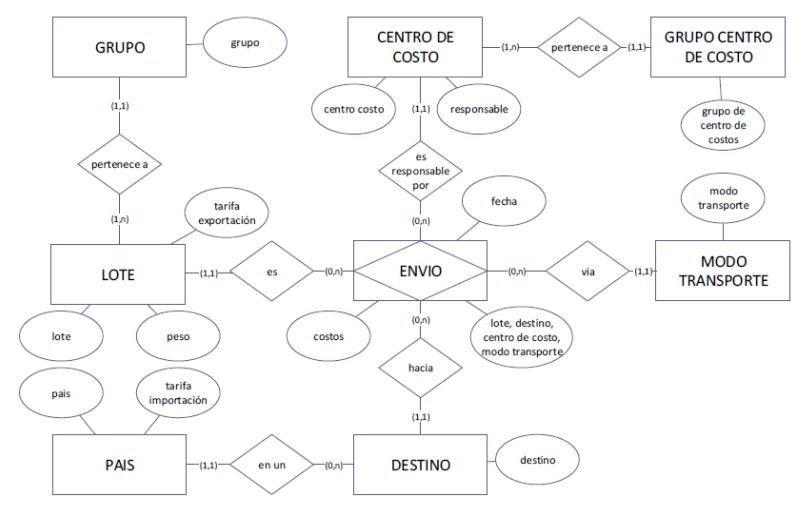
\includegraphics[width=17cm]{./Imagenes/ejercicio1}
	\end{center}	

Supongamos que los costos de los atributos ya incluyen todas las tarifas. No se transferirá más información sobre las tarifas
al almacén de datos. El análisis tendrá lugar a nivel del grupo de centros de costos, no se necesita información sobre los
centros de costos.
Por favor identifique el hecho de interés y construya el Modelo Dimensional y su respectivo diagrama físico.
\\

\begin{itemize}
    \item \textbf{Modelo Dimensional}
\\
El diseñador de software ERWIN permite que se pueda crear y modificar diagramas con facilidad, mejorando la calidad de los diseños de software. El Modelo Dimensional es el resultado directo de la llegada del diseño de flujo de datos y análisis estructural.

	\begin{center}
	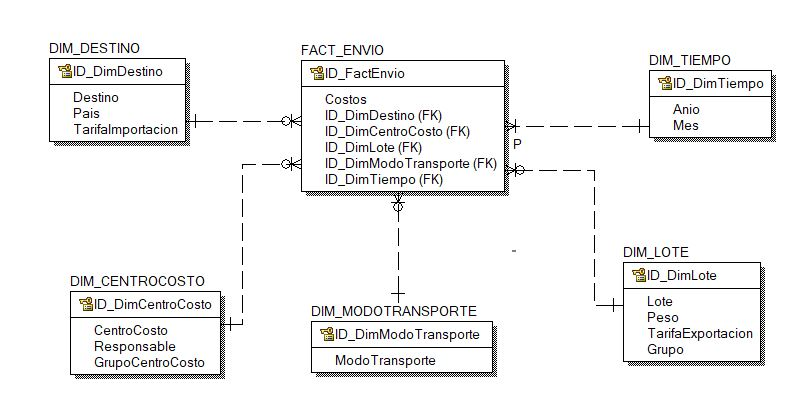
\includegraphics[width=17cm]{./Imagenes/Ejercicio1Logico}
	\end{center}	

    \item \textbf{Modelo Fisico}

Es posible crear y modificar bases de datos de forma visual a través de los diagramas de bases de Datos. Estos diagramas fisicos proporcionan una visión gráfica de las tablas en la base de datos incluyendo sus columnas, el modelo E/R y el diagrama fisico de estructura de datos en SQL Server.

	\begin{center}
	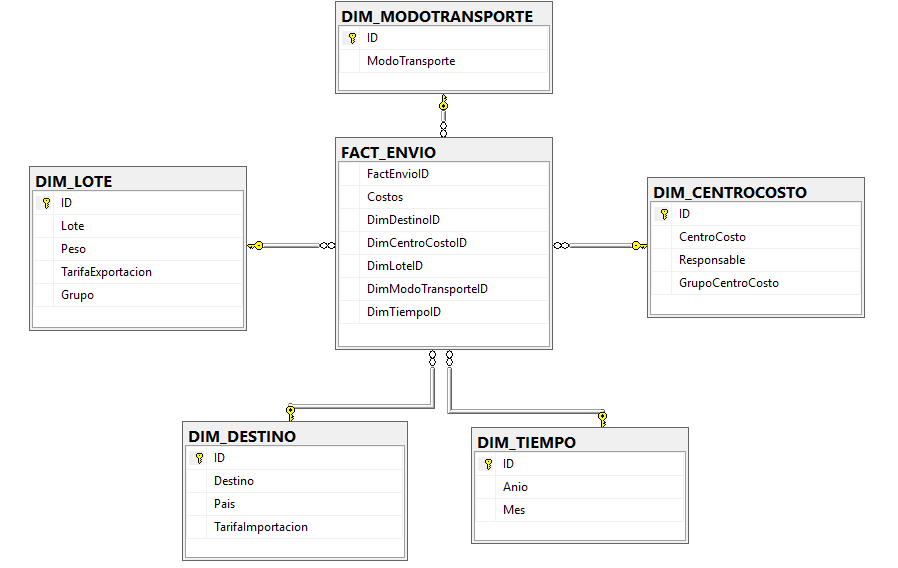
\includegraphics[width=17cm]{./Imagenes/Ejercicio1Fisico}
	\end{center}	

    \item \textbf{Código del Modelo Fisico}

	\begin{center}
	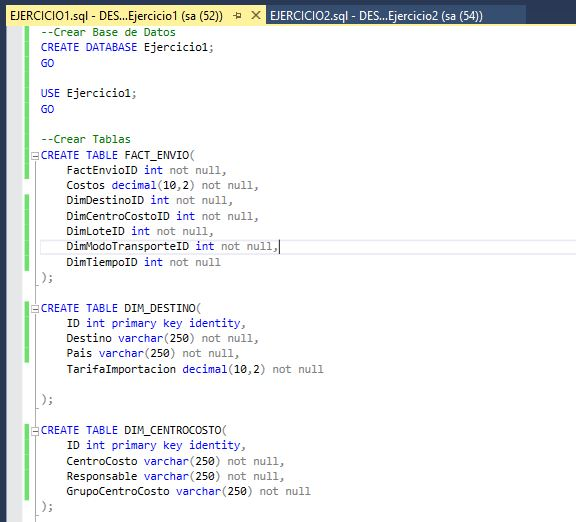
\includegraphics[width=17cm]{./Imagenes/Ejercicio1Fisico1}
	\end{center}	

	\begin{center}
	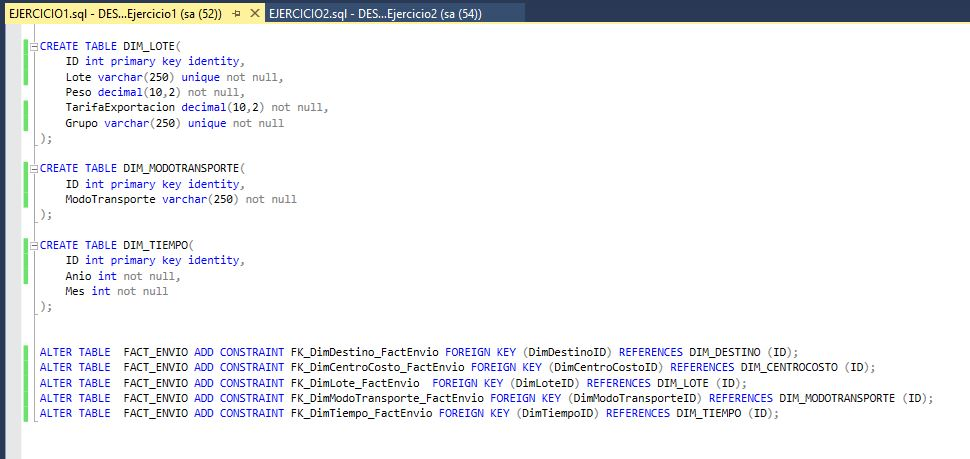
\includegraphics[width=17cm]{./Imagenes/Ejercicio1Fisico2}
	\end{center}	
\end{itemize}